\chapter{电力系统的脆弱性仿真实验与量化分析}
\label{cha:quantiAnaly}

\section{引言}
\label{sec:index5}
依据第四章所建立的电网脆弱性量化评价模型,本章以$IEEE118$标准电网为例,在系统模型的基础上,采用静态分析法研究不同攻击策略对电网结构脆弱性的影响,找出最佳的攻击策略,并验证电力系统的网络特性。
以$IEEE39$标准电网为例,分别进行仿真实验研究电力系统的结构脆弱性和状态脆弱性,最后得到系统综合脆弱性评价结果,并与其它评价模型进行对比,验证本文所建立的评价模型的科学性。
\section{基于复杂网络模型结构脆弱性实验验证分析}
\label{sec:modelIntroduce}

\subsection{电网结构脆弱性研究方法}
\label{sec:modelIntroduce}
电网作为一个复杂的人造网络,存在一些固有的缺陷或薄弱环节,当这些薄弱环节遭到破坏时,由于电网节点间的连通性,可能会导致电网运行失稳,引发电网大面积瘫痪。在结构上看,这些缺陷或薄弱环节可视为
电网的脆弱环节,因此电网脆弱环节的脆弱程度可以表征电网结构脆弱性。

从复杂网络的角度来看,研究电网结构脆弱性的基本方法为通过移除部分节点或线路来考察电网结构和功能的影响程度。电网结构脆弱性的研究方法分为静态分析法和动态分析法,其主要区别在于移除节点或线路
后是否考虑所引起的级联反应。静态分析法通过不同的电网攻击策略,分析其对电网结构连通性及传输效率的影响程度,不考虑节点或线路移除后引起的级联反应。动态分析法则考虑的是节点或线路移除后潮流分布
变化所引起的级联反应,通过建立连锁故障模型来模拟电网结构性能的动态变化。由于本文对电网结构脆弱性的重点在于识别系统的薄弱环节,选取最优攻击策略,所以在研究方法上,采用静态分析法。 

\subsection{指标选取及元件攻击策略的制定}
\label{sec:modelIntroduce}
为识别电力系统的脆弱环节并找到最优的攻击策略,需要制定电网的攻击策略以及选取电网整体性能指标,从电网结构拓扑方面考虑,网络传输效率是用于描述电网能量传输的重要性能指标。为此,本文选取第二章所述
的网络平均传输效率$E_{mean}$作为电网结构性能评价指标。

在第三章中,通过对结构脆弱性的研究,得到电气度、电气介数和$PageRank$值这三个指标作为结构脆弱性指标,为比较这三个指标对于电网结构性能的影响程度,分别按照式\ref{equ:chap3:index1},式\ref{equ:chap3:cb1}
和式\ref{equ:chap3:Index3}计算$IEEE118$算例中各节点的电气度、电气介数$PageRank$值,并将各节点的计算结果进行排序。下面将围绕电气度、电气介数$PageRank$值这三个指标指定攻击策略,观察比较
电网结构性能指标的变化情况,并引入随机节点攻击策略作为实验对比。具体策略如下:

$(1)$随机节点攻击策略——每次随机移除1个节点,移除比例为30$\%$,仿真100次,取性能指标结果的平均值;

$(2)$电气度节点攻击策略——每次移除电气度值最大的节点,移除比例为30$\%$,记录每次的性能指标仿真结果;

$(3)$电气介数节点攻击策略——每次移除电气介数值最大的节点,移除比例为30$\%$,记录每次的性能指标仿真结果;

$(4)$$PageRank$值节点攻击策略——每次移除$PageRank$值最大的节点,移除比例为30$\%$,记录每次的性能指标仿真结果;



\subsection{实验仿真与分析}
\label{sec:modelIntroduce}
本文采用的$IEEE118$标准算例数据见附录A所示,其中各节点电气度、电气介数和$PageRank$值计算结果,分别如图\ref{fig:electricDu118},\ref{fig:nodeBetween118}和\ref{fig:pagerank118}所示,
实验结果数据见附录B。
\begin{figure}[H] % use float package if you want it here
    \centering
    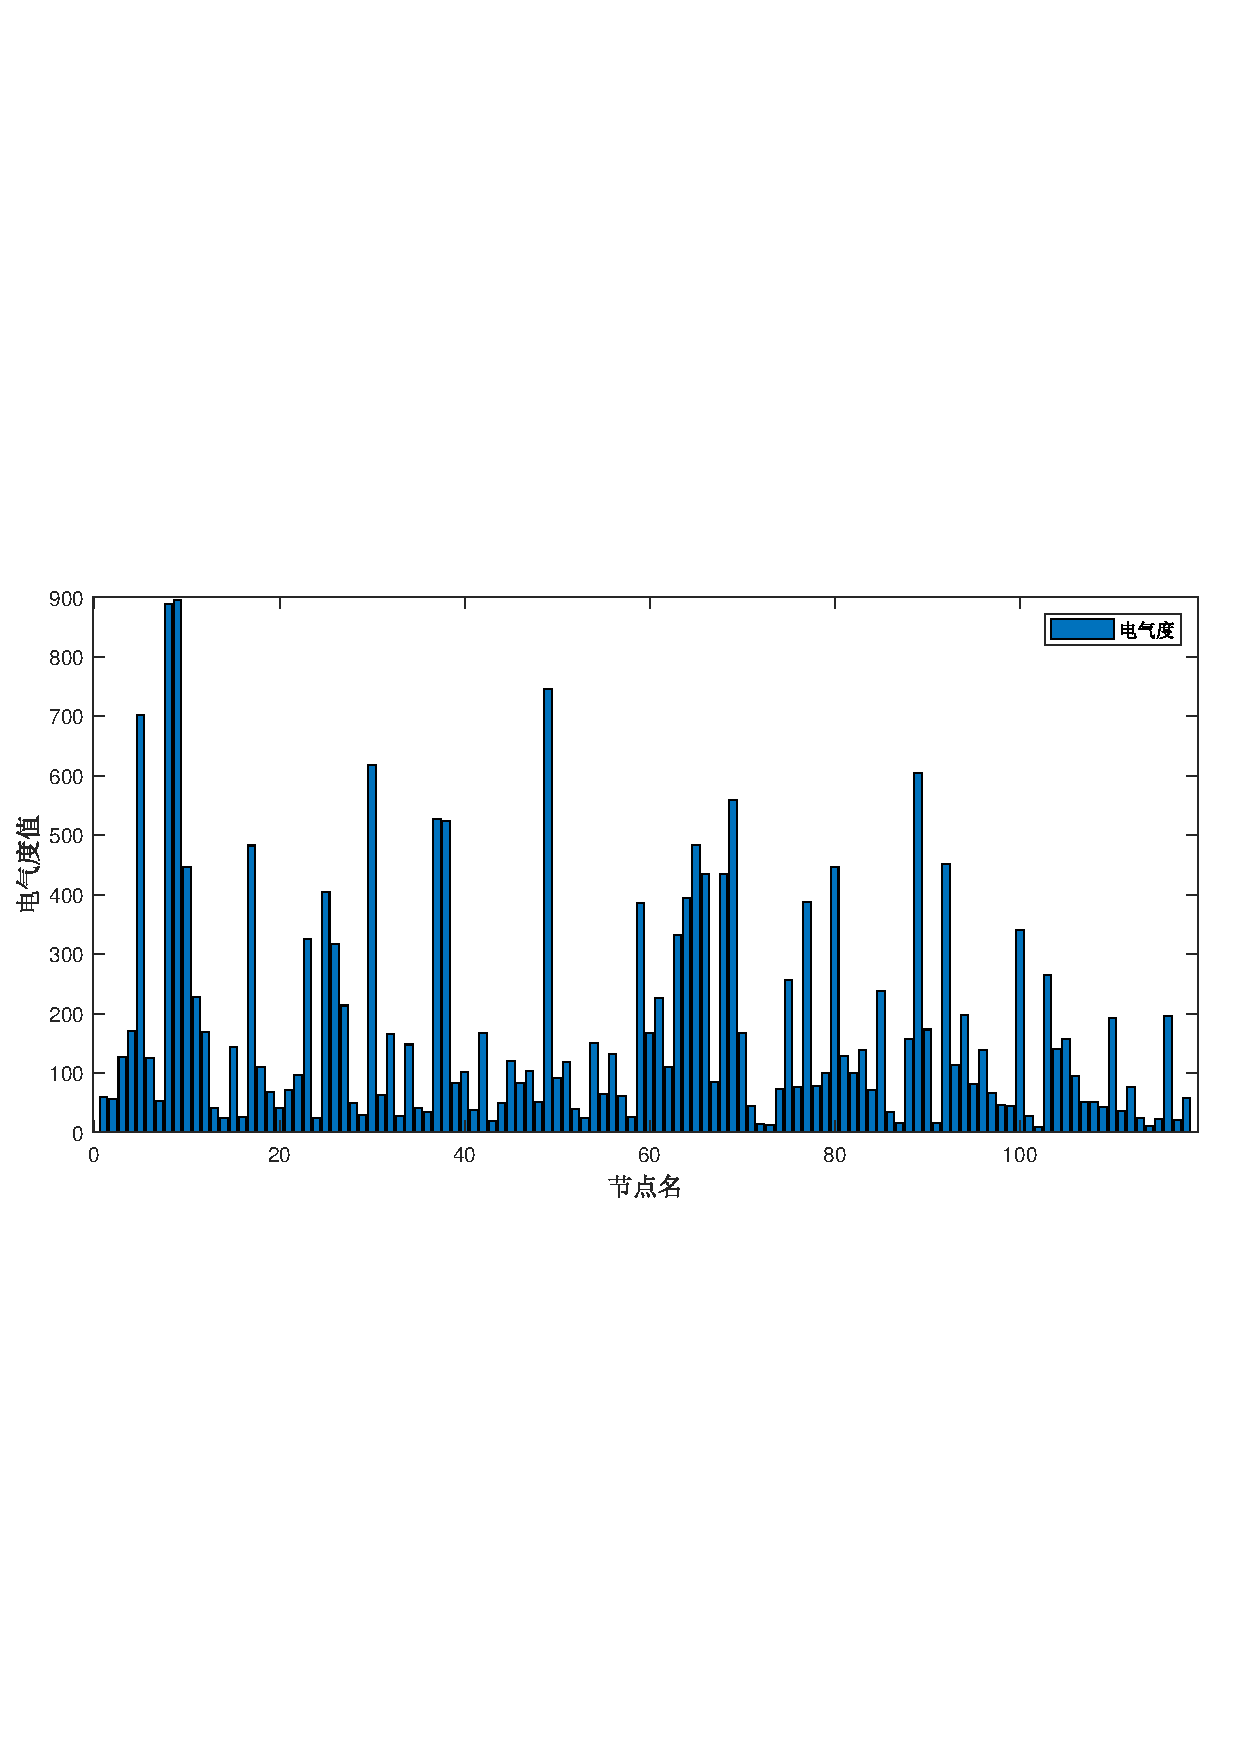
\includegraphics[width=14cm,height=7cm]{electricDu118.pdf}
    \caption{$IEEE118$节点电气度计算结果图}
    \label{fig:electricDu118}
  \end{figure}
\begin{figure}[H] % use float package if you want it here
    \centering
    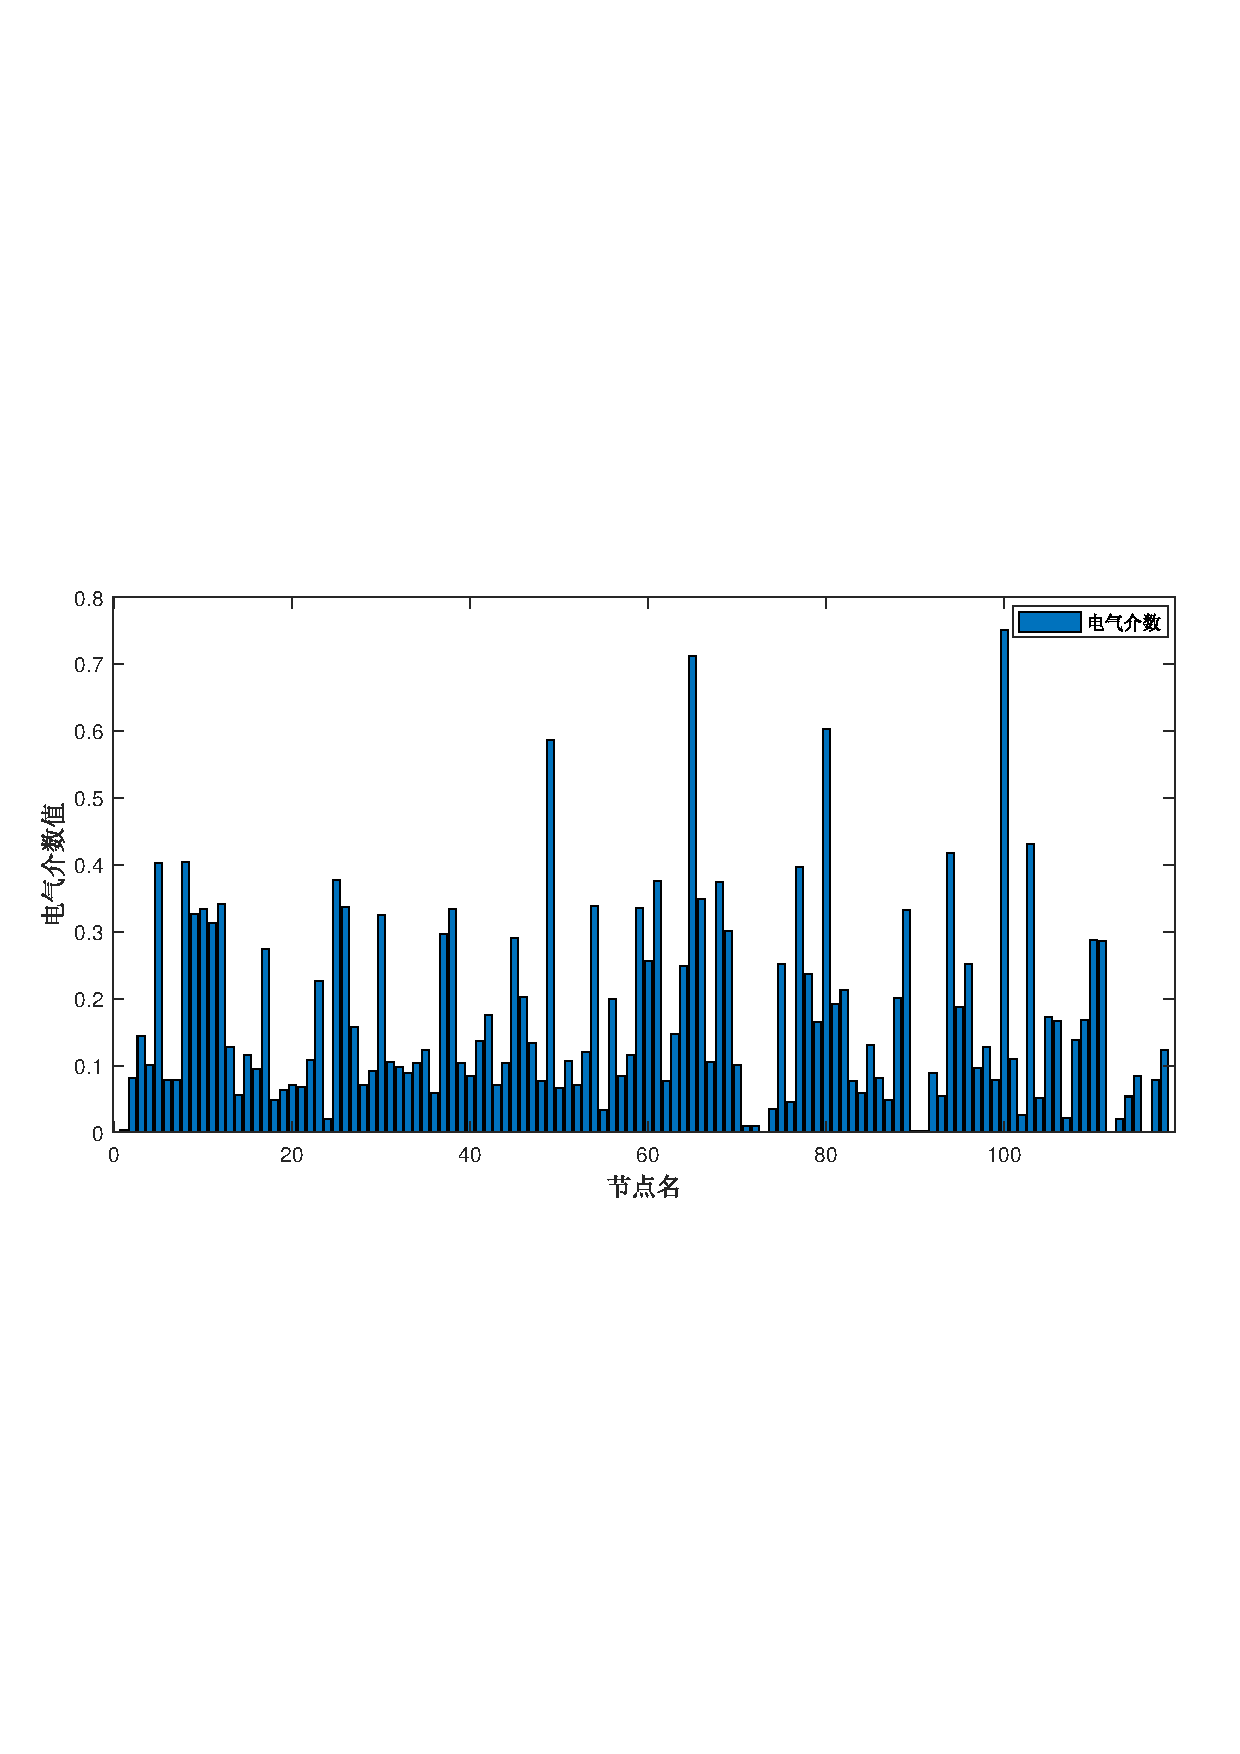
\includegraphics[width=14cm,height=7cm]{nodebetween118.pdf}
    \caption{$IEEE118$节点电气介数计算结果图}
    \label{fig:nodeBetween118}
\end{figure}
\begin{figure}[H] % use float package if you want it here
    \centering
    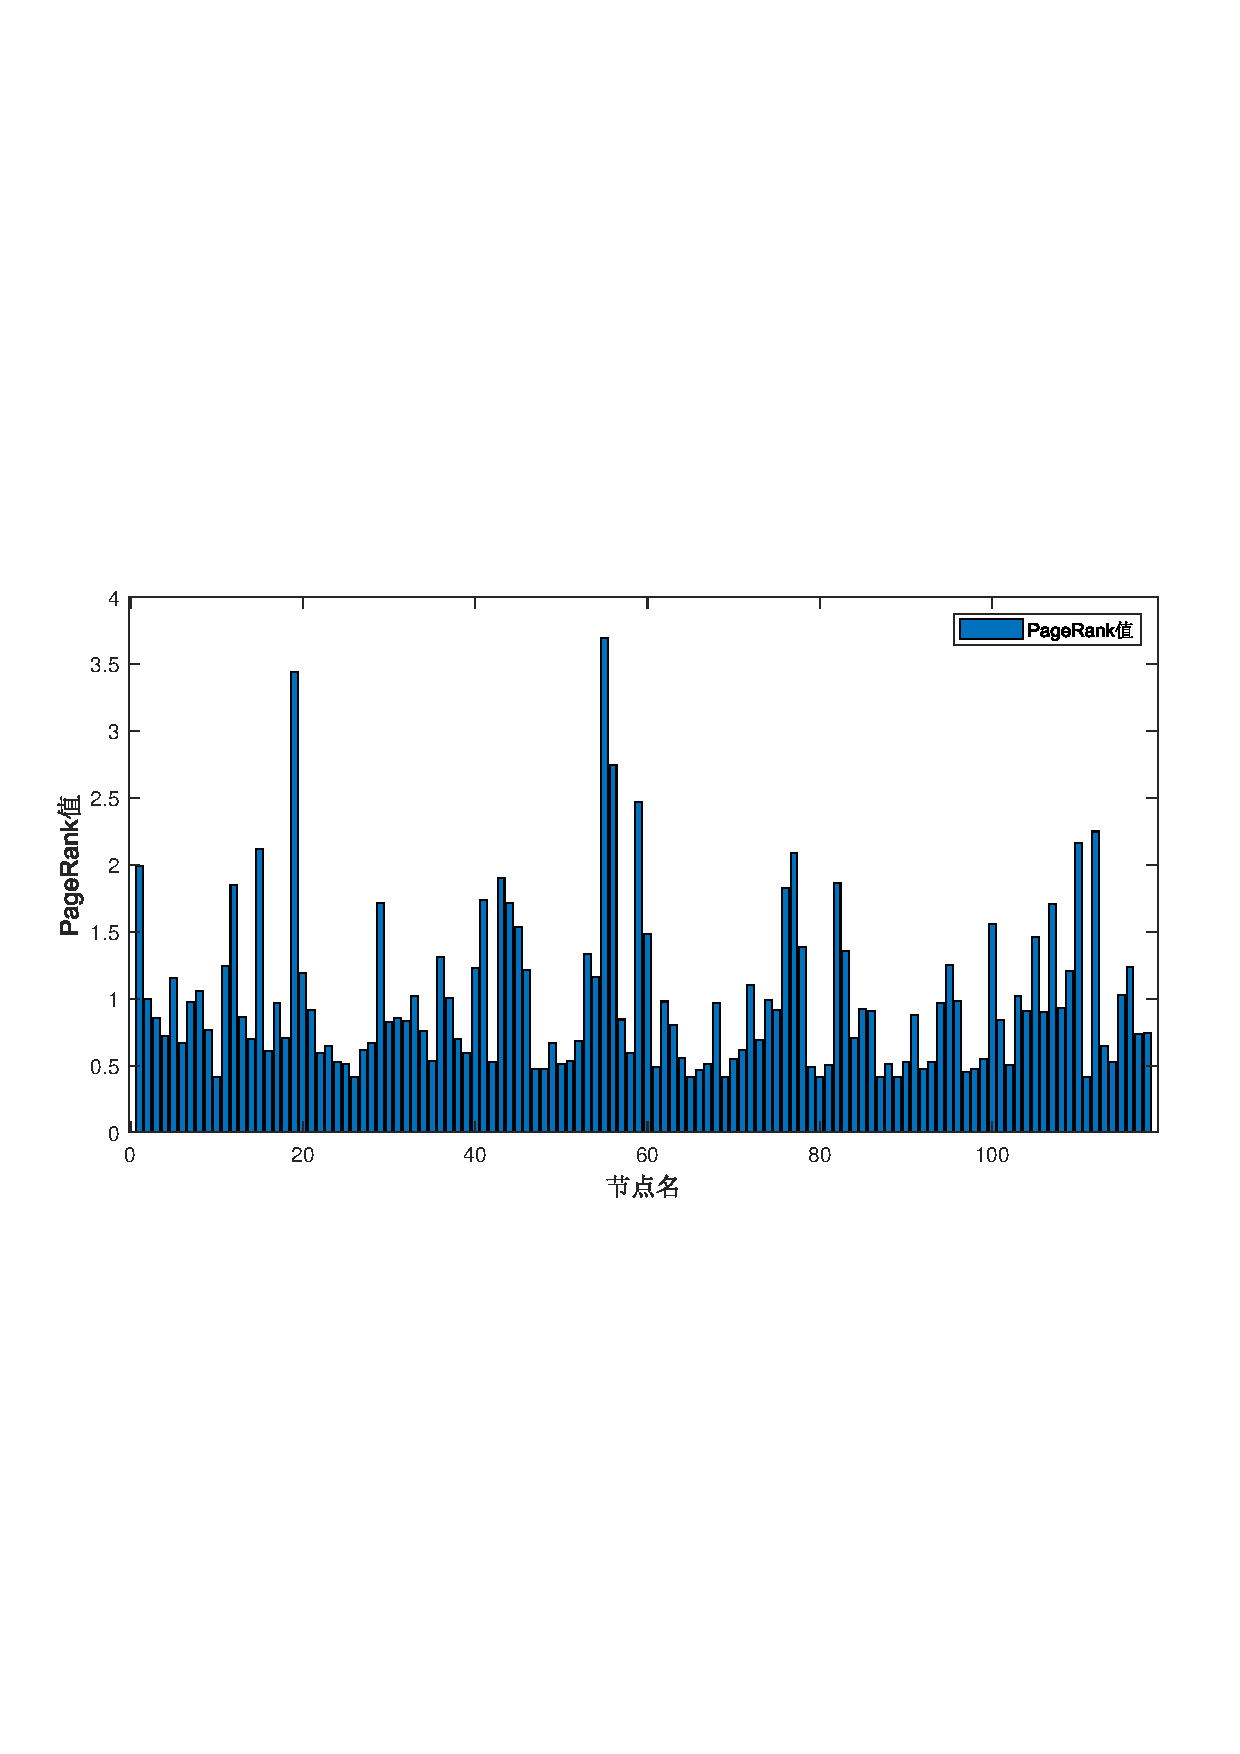
\includegraphics[width=14cm,height=7cm]{PageRank118.pdf}
    \caption{$IEEE118$节点PageRank值计算结果图}
    \label{fig:pagerank118}
\end{figure}

从图\ref{fig:electricDu118}、\ref{fig:nodeBetween118}和\ref{fig:pagerank118}可以看出,电气度指标值较高的节点名有9、8、49、5、30、89等,这些节点在电网结构中的邻接节点较多,
所连支路承担的潮流值较大;电气介数指标值较高的节点名有100、65、80、49、103等,表明电气介数值较大节点在结构和能量传输方面的重要程度高;PageRank指标值较高的节点名有1、55、19、56、59等,
这些节点的入链数目多,在潮流累计分布中比重较大。因此,在电网结构中的重要程度高。

下面为电气度、电气介数、$PageRank$值按照重要程度的节点号排名,取移除比例为$30\%$的节点数量。如表\ref{tab:rank118}所示。
\begin{table}[H]
    \centering
    \caption{电气度、电气介数、$PageRank$值节点号排名}
    \label{tab:rank118}
      \begin{tabular}{C{3cm}C{3cm}C{3cm}C{4cm}}
        \toprule
        节点排名  & 电气度节点名   & 电气介数节点名     & PageRank值节点名\\
        \midrule
        1       & 9              & 100                & 1 \\
        2       & 8              & 65                 & 55 \\
        3       & 49             & 80                 & 19 \\
        4       & 5              & 49                 & 56 \\
        5       & 30             & 103                 & 59 \\
        6       & 89             & 94                 & 112 \\
        7       & 69             & 8                 & 110 \\
        8       & 37             & 5                 & 15 \\
        9       & 38             & 77                 & 77 \\
        10      & 65             & 25                 & 43 \\
        11      & 17               & 61                & 82 \\
        12      & 92               & 68                 & 12 \\
        13      & 80               & 12                 & 76 \\
        14      & 10                 & 54                 & 41 \\
        15      & 68                 & 26                 & 44 \\
        16      & 66                 & 59                 & 29 \\
        17      & 25                 & 10                 & 107 \\
        18      & 64                 & 38                 & 100 \\
        19      & 77                 & 89                 & 45 \\
        20      & 59                 & 9                 & 60 \\
        21      & 100                & 30                 & 105 \\
        22      & 63                 & 11                 & 78 \\
        23      & 23                 & 69                 & 83 \\
        24      & 26                 & 37                 & 53 \\
        25      & 103                & 45                 & 36 \\
        26      & 75                 & 110                 & 95 \\
        27      & 85                 & 111                 & 11 \\
        28      & 11                 & 17                 & 116 \\
        29      & 61                 & 60                 & 40 \\
        30      & 27                 & 75                 & 46 \\
        31      & 94                 & 96                 & 109 \\
        32      & 116                 & 64                 & 20 \\
        33      & 110                 & 78                 & 54 \\
        34      & 90                 & 23                 & 5 \\
        35      & 4                 & 82                 & 72 \\
        36      & 12                 & 46                 & 8 \\
        37      & 60                & 88                 & 115 \\
        38      & 70                 & 56                 & 33 \\
        39      & 42                & 81                 & 103 \\
        \bottomrule
      \end{tabular}
\end{table}

下面为四种攻击策略下的仿真结果,如图\ref{fig:chap5:4Efficiency118}、\ref{fig:chap5:Efficiency118}所示。
\begin{figure}[H] % use float package if you want it here
  \centering
  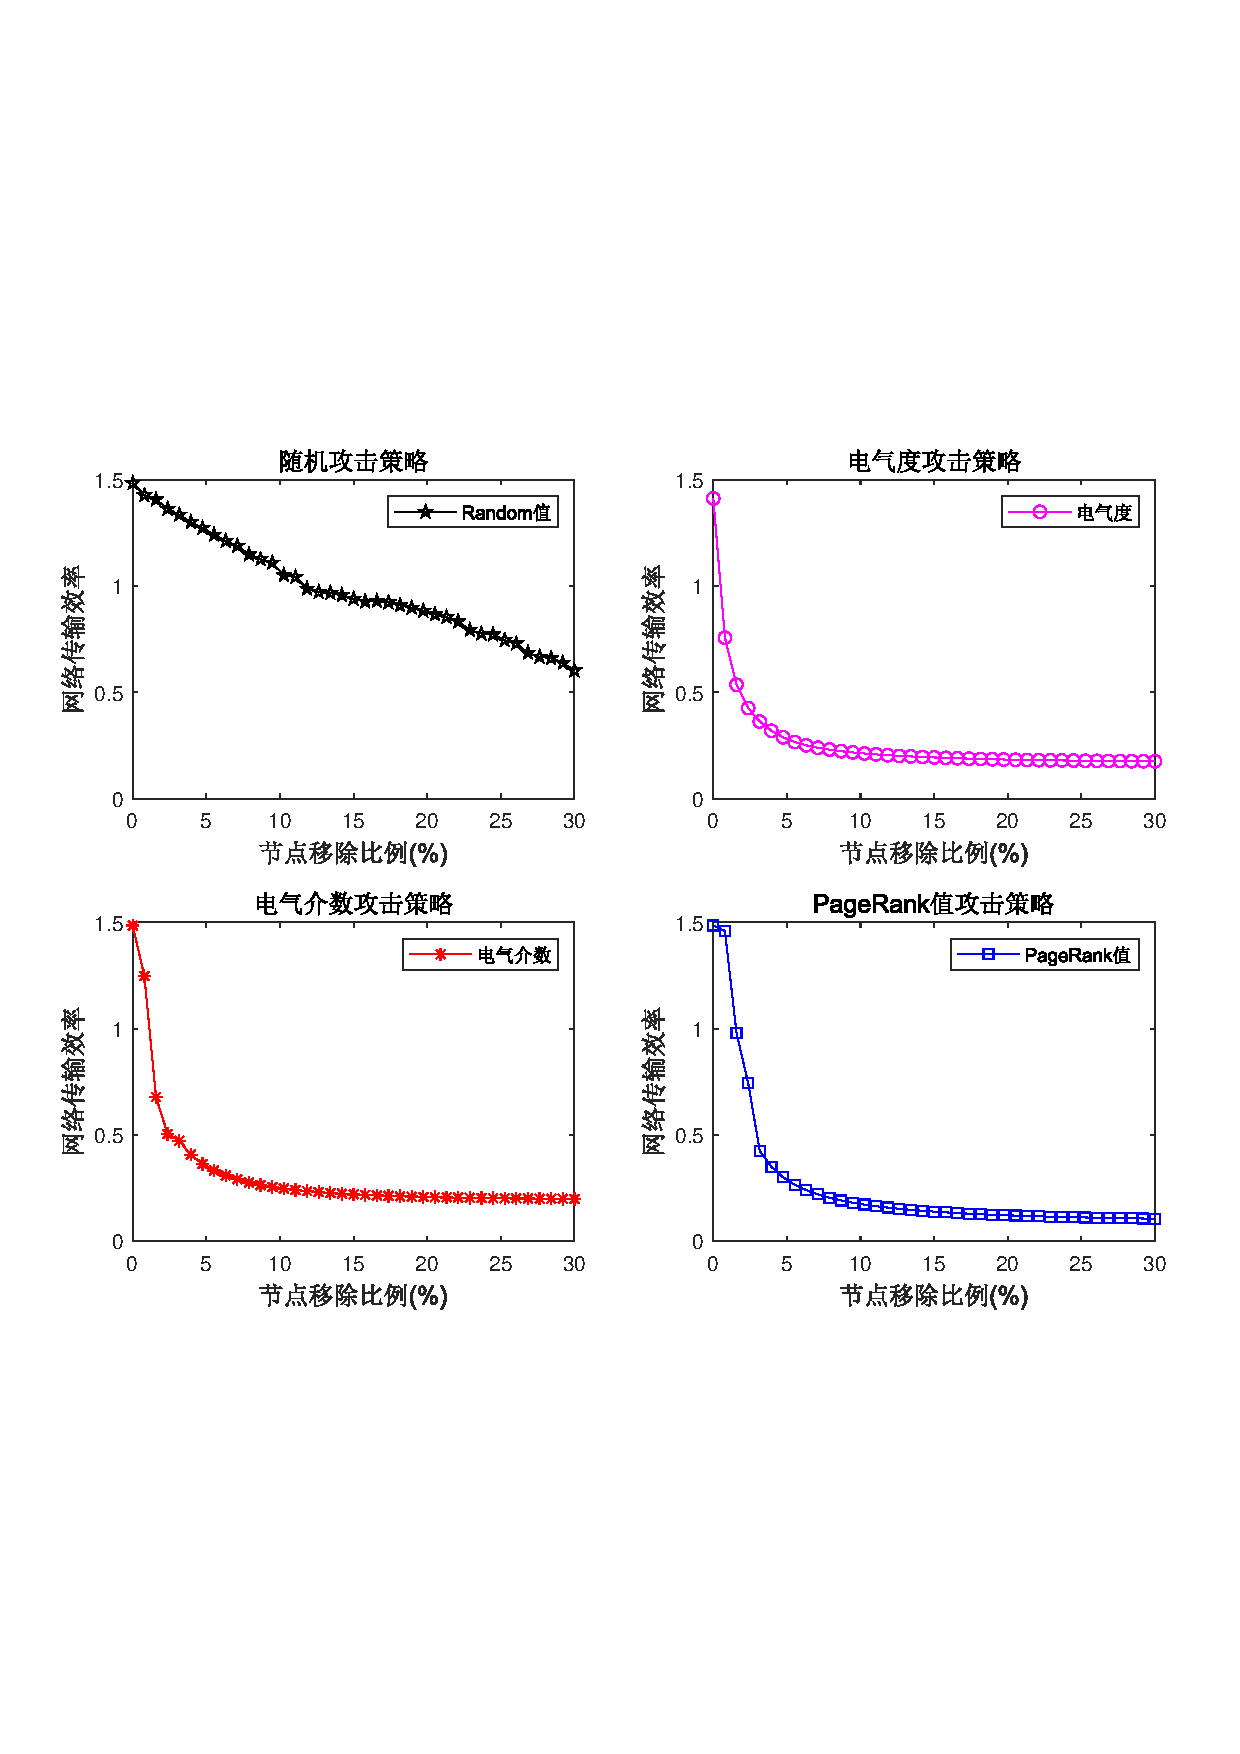
\includegraphics[width=13.4cm,height=9.6cm]{4Efficiency118.pdf}
  \caption{四种攻击策略下电网平均传输效率趋势图}
  \label{fig:chap5:4Efficiency118}
\end{figure}
\begin{figure}[H] % use float package if you want it here
  \centering
  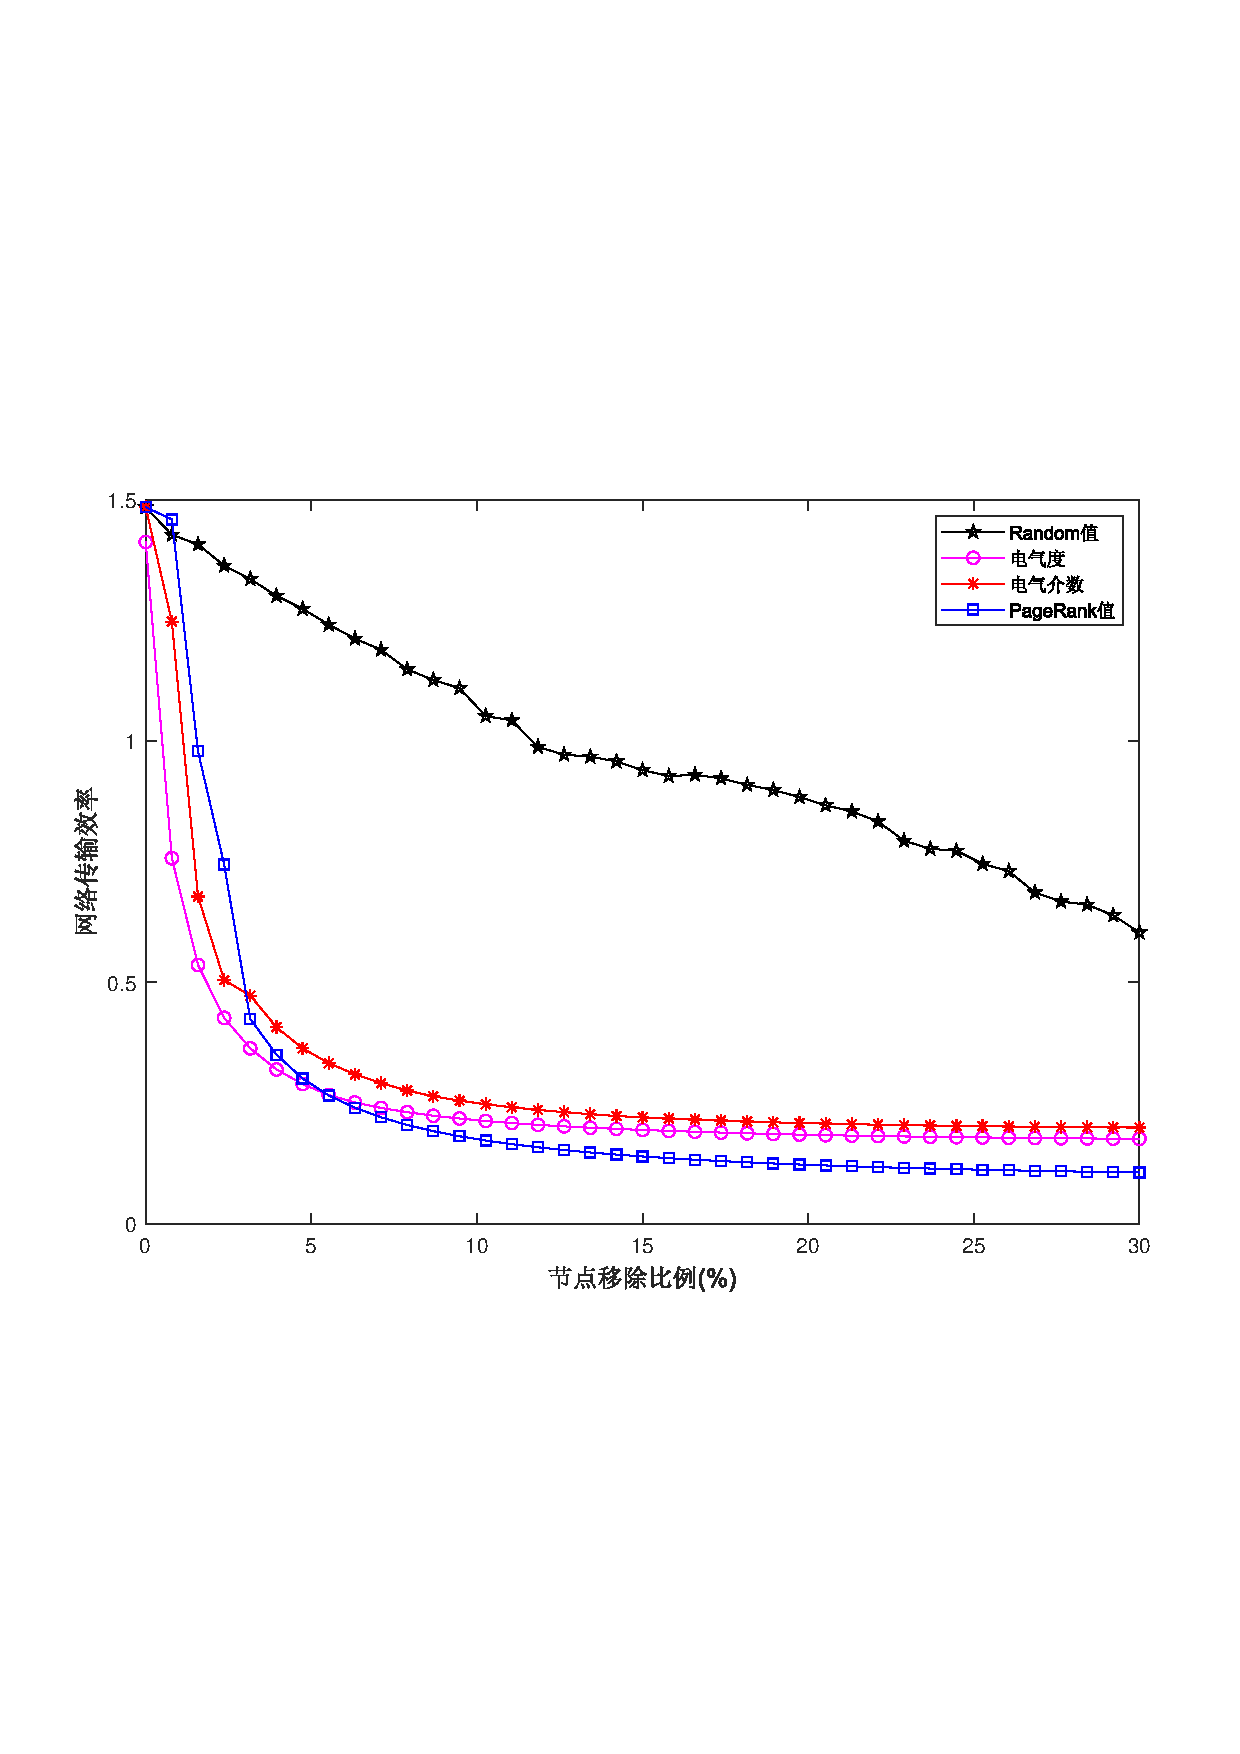
\includegraphics[width=13.4cm,height=9.1cm]{Efficiency118.pdf}
  \caption{四种电网攻击策略结果对比图}
  \label{fig:chap5:Efficiency118}
\end{figure}

从图\ref{fig:chap5:4Efficiency118}、\ref{fig:chap5:Efficiency118}的实验结果可以看出:

$(1)$在随机攻击策略下,网络传输效率值下降较为平缓,在节点移除比例至$30\%$时,电网的传输效率约为原来传输效率的$40\%$。而与其他三种攻击策略相比,
电气度、电气介数和$PageRank$值攻击策略对于电网传输效率的破坏性更高,在移除比例约为$10\%$时,电网平均传输效率已分别降至原来的$14.9\%$、$17.6\%$和$12.8\%$。因此,本文基于复杂网络
理论得到的脆弱性指标可以科学合理地描述系统各节点在电网中的重要程度,并可进一步衡量各节点在电网中的脆弱性。

$(2)$随机攻击策略对于电网的连通性影响较小,而蓄意攻击将会对网络连通性及传输效率影响较大,说明电网对于随机攻击具有很好的鲁棒性,进一步证实了电网的无标度性。

$(3)$对比三种蓄意攻击策略,从图\ref{fig:chap5:Efficiency118}得到,在节点移除前期,电气度攻击对于电网平均传输效率下降趋势最为明显,其原因在于,电气度是基于节点度进行定义的,电气度
指标更多的是专注于电网拓扑结构的重要性。在电气度的攻击策略下,节点的移除时意味着最大程度切断其他节点与所移除节点的联系,这将极大地破坏电网的拓扑结构,进而影响电网传输性能。可以证实,
电网拓扑结构的稳定性是电力系统正常运行的重要保证和前提条件,其节点的分布和联系是影响电网脆弱性的重要因素。在节点移除的后期,电气度、电气介数和$PageRank$值攻击策略对电网传输效率值分别
下降为$11.71\%$、$13.26\%$、$7.06\%$,在后期的移除过程中,$PageRank$值攻击策略的破坏性更高,原因在于,$PageRank$值指标关注的是潮流流向对于电网结构的重要性,指向节点的潮流数越多意味着
此节点的重要性越高,按照此攻击策略进行移除,将会导致发电节点所传输的功率所供给的节点越来越少,传输效率下降,直至无法进行功率传输。

综上分析,电气度、电气介数和$PageRank$的攻击策略相较于随机攻击策略的破坏性较大,从而验证了这三种指标可作为脆弱性指标的合理性,通过三种蓄意攻击策略的对比,可得到电气度专注于电网结构拓扑的
重要性,PageRank值则侧重于节点入链数的重要性,而电气介数综合考虑节点支路和支路潮流对电网结构的影响程度,其对电网的破坏性较为均衡。



\section{电力系统脆弱性分析评估}
\label{sec:singleAssessment}




\subsection{电力系统结构脆弱性实验分析}
\label{sec:singleAnalysis_fabric}




\subsection{电力系统状态脆弱性实验分析}
\label{sec:singleAnalysis_status}





\subsection{电力系统综合脆弱性分析}
\label{sec:singleAnalysis}





\section{电力系统脆弱性等级评估}
\label{sec:multiAssessment}




\subsection{基于聚类算法的电力系统脆弱等级评估}
\label{sec:multiVSsingle}




\subsection{基于综合指标排序的电力系统脆弱等级评估}
\label{sec:multiAnalysis}





\subsection{结果分析与比较}




\section{本章小结}
\label{sec:sum5}


